% pre-report.tex — รายงานฉบับย่อ แปลงจาก pre-report.md (รูปแบบ paper สากล + ย่อหน้าแบบไทย)
%   ทุกประโยคตรวจกับ presentation/data/facts.json, data/processed/ และ report.md
%   บันทึกการตรวจ (ข้อความเดิม → ที่แก้ → หลักฐาน) อยู่ใน pre-report-claimcheck.md
%   คอมไพล์:  cd reports/final && latexmk -xelatex pre-report.tex
%   รูปทั้งหมดมาจาก figures/report/ (สร้างด้วย scripts/make_figures.py และ scripts/make_infographics.py)
\documentclass[a4paper,11pt]{article}

\usepackage[a4paper,margin=2.5cm]{geometry}
\usepackage{amsmath}
\usepackage{unicode-math}
\usepackage{booktabs}
\usepackage{array}
\usepackage{tabularx}
\usepackage{xcolor}
\usepackage{enumitem}
\usepackage{caption}
\usepackage{graphicx}
\usepackage{float}
\usepackage{tikz}
\usetikzlibrary{arrows.meta,calc}
\usepackage{indentfirst}   % ย่อหน้าแรกหลังหัวข้อต้องย่อด้วย (LaTeX ปกติไม่ย่อ แต่แบบไทยย่อทุกย่อหน้า)
\usepackage[hidelinks]{hyperref}

\graphicspath{{../../figures/report/}}

% ---------- ฟอนต์แบบ paper สากล ----------
% อักษรละตินและคณิตศาสตร์ใช้ Times (TeX Gyre Termes) ส่วนอักษรไทยสลับไปใช้ Noto Serif Thai อัตโนมัติ
% ด้วยกลไก interchar ของ XeTeX (ตรวจ Unicode block ของแต่ละตัวอักษร) — ตัวหนา/เอียงยังคงตามบริบทเดิม
\setmainfont{TeX Gyre Termes}
\setmathfont{TeX Gyre Termes Math}
\setmonofont{DejaVu Sans Mono}[Scale=0.78]
\newfontfamily\thaifont{Noto Serif Thai}[Script=Thai,Scale=0.92,ItalicFont={Noto Serif Thai},BoldItalicFont={Noto Serif Thai Bold}]  % อักษรไทยไม่มีตัวเอียง ใช้ตัวตรงแทน
\newfontfamily\symbolfont{DejaVu Sans}   % สำหรับอักขระ ✓
\newcommand{\tick}{{\symbolfont ✓}}
% กำหนดอักษรไทย U+0E00–U+0E7F เป็นคลาสหนึ่ง แล้วสลับฟอนต์ทุกครั้งที่ข้ามระหว่างไทยกับอักขระอื่น
% คลาส 0 = อักขระทั่วไป (ละติน ตัวเลข วรรคตอน) · คลาส 4095 = ขอบ (ช่องว่าง ต้นกลุ่ม ฯลฯ)
\makeatletter
\newXeTeXintercharclass\thaicharclass
\@tempcnta="0E00
\loop\ifnum\@tempcnta<"0E80
  \XeTeXcharclass\@tempcnta=\thaicharclass
  \advance\@tempcnta by 1
\repeat
\makeatother
\XeTeXinterchartokenstate=1
\XeTeXinterchartoks 0 \thaicharclass = {\thaifont}
\XeTeXinterchartoks 4095 \thaicharclass = {\thaifont}
\XeTeXinterchartoks \thaicharclass 0 = {\rmfamily}
\XeTeXinterchartoks \thaicharclass 4095 = {\rmfamily}
\XeTeXlinebreaklocale "th"       % ตัดคำไทยด้วย ICU (ภาษาไทยไม่มีช่องว่างระหว่างคำ)
\XeTeXlinebreakskip = 0pt plus 0.25pt
\tolerance=6000 \emergencystretch=4em \hbadness=4000
\linespread{1.12}

% ---------- ย่อหน้าแบบไทย: ย่อบรรทัดแรกทุกย่อหน้า ----------
\setlength{\parindent}{1.27cm}
\setlength{\parskip}{0pt plus 1pt}

% ---------- รายการ ----------
\setlist[enumerate]{before=\raggedright,leftmargin=*,labelindent=\parindent,itemsep=0.1em,topsep=0.2em,parsep=0pt}
\setlist[itemize]{leftmargin=*,labelindent=\parindent,itemsep=0.1em,topsep=0.2em,parsep=0pt}

% ---------- คำบรรยายรูป/ตาราง ----------
\captionsetup{font=small,labelfont=bf,labelsep=colon,skip=6pt}
\captionsetup[figure]{name=รูปที่}
\captionsetup[table]{name=ตารางที่,position=top}

% ---------- ตาราง ----------
\renewcommand{\arraystretch}{1.2}
\newcolumntype{L}[1]{>{\raggedright\arraybackslash}p{#1}}
\newcolumntype{Y}{>{\raggedright\arraybackslash}X}

% หัวข้อไม่มีเลข (เอกสารอ้างอิง)
\newcommand{\centerheading}[1]{\section*{#1}}

\begin{document}

% ======================================================================
%  ชื่อเรื่อง ผู้แต่ง บทคัดย่อ (ถ้อยคำคงตาม pre-report.md · แก้เฉพาะ claim ที่ผิด/ขาดอ้างอิง
%  ดูบันทึกใน pre-report-claimcheck.md)
% ======================================================================
\begin{center}
{\LARGE\bfseries ความสัมพันธ์เชิงเวลา–คาบระหว่างความผันแปรระหว่างปีของระดับน้ำทะเล%
ชายฝั่งประเทศไทยกับดัชนีภูมิอากาศด้วย Wavelet Coherence และ Multiple Wavelet Coherence\par}
\vspace{0.8em}
{\large\bfseries\itshape Time–Scale Relationships between Interannual Sea-Level Variability along the Thai Coasts
and Climate Indices: An Analysis Using Wavelet Coherence and Multiple Wavelet Coherence\par}
\vspace{1.2em}
{\large กวินภพ จันเจือ (รหัสนิสิต 6710503739)\par}
\vspace{0.3em}
{\small ภาควิชาวิศวกรรมคอมพิวเตอร์\\
รายงานโครงงานรายวิชา 01204496 การประมวลผลสัญญาณดิจิทัลเชิงอัลกอริทึมสำหรับวิศวกรคอมพิวเตอร์\\
ตุลาคม 2569\par}
\end{center}

\vspace{0.6em}
\begin{center}\bfseries บทคัดย่อ\end{center}
\vspace{-0.6em}
\begin{quote}\small
การศึกษานี้วิเคราะห์ความสัมพันธ์ระหว่างความผันแปรระหว่างปีของระดับน้ำทะเลที่สถานีเกาะตะเภาน้อย (ทะเลอันดามัน)
และเกาะหลัก (อ่าวไทย) กับดัชนีภูมิอากาศ 8 ตัวในช่วง ค.ศ. 1951–2023 ด้วยเครื่องมือ wavelet coherence (WTC)
และ multiple wavelet coherence (MWC) โดยได้ประเมินระดับนัยสำคัญจากการจำลองมอนติคาร์โลและปรับเกณฑ์ตามจำนวนดัชนีที่ใช้งานอย่างรัดกุม
ผลการศึกษาพบว่าระดับน้ำทะเลที่เกาะตะเภาน้อยสัมพันธ์อย่างมีนัยสำคัญกับดัชนี SOI, DMI, WNPMI และ Niño3.4
สอดคล้องกับกลไกของคลื่นเคลวิน ในขณะที่ระดับน้ำทะเลที่เกาะหลักไม่พบความสัมพันธ์กับดัชนีใดเกินกว่าระดับสัญญาณรบกวน
นอกจากนี้ การใช้ MWC รวมดัชนีหลายตัวไม่ได้เพิ่มอำนาจอธิบายมากไปกว่าการใช้ดัชนีเดี่ยว หากมีการปรับเกณฑ์นัยสำคัญอย่างเหมาะสม
ข้อมูลมาตรวัดที่เกาะตะเภาน้อยจากสองคลังข้อมูลมีความไม่สอดคล้องกันหลังปี ค.ศ. 2005
ทำให้ไม่สามารถระบุลำดับความสำคัญของดัชนีในช่วงคาบ 2–7 ปีได้อย่างแน่ชัด

\vspace{0.5em}
\noindent\textbf{คำสำคัญ:} ระดับน้ำทะเล, wavelet coherence, multiple wavelet coherence, ENSO, Indian Ocean Dipole,
ทะเลอันดามัน, อ่าวไทย
\end{quote}
\vspace{0.5em}

% ======================================================================
\section{บทนำ}

\subsection{ที่มาและความสำคัญ}

ระดับน้ำทะเลประกอบด้วยหลายองค์ประกอบที่ซ้อนทับกัน เช่น วงรอบฤดูกาล ความผันแปรระหว่างปี (การเปลี่ยนแปลงที่เกิดขึ้นข้ามปี)
และแนวโน้มระยะยาว (การเปลี่ยนแปลงระดับน้ำสะสมในระยะหลายปี) องค์ประกอบระหว่างปีมีความไม่คงที่ (non-stationary)
จึงทำให้เครื่องมือทางสถิติที่อาศัยค่าเฉลี่ยตลอดอนุกรมเวลาไม่สามารถจับรูปแบบความสัมพันธ์ได้ดีนัก
การแปลงเวฟเล็ตจึงเป็นเครื่องมือที่เหมาะสมกว่า (Torrence \& Compo, 1998) งานวิจัยต้นทาง (Song \& Chen, 2022)
ใช้ WTC และ MWC กับข้อมูลระดับน้ำทะเล แต่ไม่ได้ระบุชัดเจนถึงการปรับเกณฑ์นัยสำคัญตามจำนวนดัชนี
รวมถึงยังไม่พบการนำวิธีนี้มาใช้กับชายฝั่งประเทศไทย ซึ่งมีลักษณะภูมิศาสตร์แตกต่างกันชัดเจนระหว่างฝั่งทะเลอันดามันและอ่าวไทย

\subsection{วัตถุประสงค์}

\begin{itemize}
  \item เพื่อวิเคราะห์ความสัมพันธ์ระหว่างระดับน้ำทะเลชายฝั่งไทยกับดัชนีภูมิอากาศด้วย WTC และ MWC
  \item เพื่อเปรียบเทียบการตอบสนองของระดับน้ำทะเลฝั่งทะเลอันดามันและอ่าวไทย
  \item เพื่อประเมินผลของการปรับเกณฑ์นัยสำคัญตามจำนวนดัชนีในแบบจำลอง MWC
  \item เพื่อตรวจสอบความถูกต้องของการลดอัตราสุ่มข้อมูลระดับน้ำทะเลเทียบกับข้อมูลอ้างอิง
\end{itemize}

\subsection{คำถามการวิจัย}

\begin{table}[H]
\caption{คำถามการวิจัยและหัวข้อที่ตอบคำถาม}\label{tab:rq}
\centering\small
\begin{tabularx}{\textwidth}{@{}l Y l@{}}
\toprule
\textbf{รหัส} & \textbf{คำถามการวิจัย} & \textbf{หัวข้อ} \\
\midrule
Q1 & ดัชนีภูมิอากาศเดี่ยวตัวใดสัมพันธ์กับระดับน้ำทะเลมากที่สุด และที่คาบใด & 4.2 \\
Q2 & ระดับน้ำทะเลฝั่งทะเลอันดามันและฝั่งอ่าวไทยตอบสนองต่อดัชนีภูมิอากาศแตกต่างกันหรือไม่ & 4.2–4.3 \\
Q3 & จำนวนดัชนีที่จำเป็นต่อการอธิบายระดับน้ำทะเลคือเท่าใด & 4.7 \\
Q4 & ชุดดัชนีใดอธิบายระดับน้ำทะเลได้ดีที่สุด & 4.7 \\
Q5 & ดัชนีประจำภูมิภาค (DMI, WNPMI) เพิ่มอำนาจอธิบายเหนือดัชนีหกตัวของงานต้นทางหรือไม่ & 4.7 \\
Q6 & การเพิ่มขึ้นของ PASC ตามจำนวนดัชนีสะท้อนความสัมพันธ์จริงเพียงใด & 4.6 \\
Q7 & อนุกรมรายเดือนที่ได้จากการกรองและลดอัตราสุ่มสอดคล้องกับข้อมูลของ PSMSL หรือไม่ & 4.1 \\
Q8 & สถานีป้อมพระจุลจอมเกล้าซึ่งได้รับผลจากการทรุดตัวของแผ่นดินให้ผลแตกต่างจากสถานีอื่นหรือไม่ & 4.3 \\
\bottomrule
\end{tabularx}
\end{table}

\subsection{ขอบเขตการศึกษา}

\begin{itemize}
  \item ศึกษาความผันแปรระหว่างปีของข้อมูลระดับน้ำทะเลรายเดือน (ม.ค. 1951 ถึง ม.ค. 2023 สิ้นสุดตามความพร้อมของข้อมูล AMO)
  \item ใช้ข้อมูลจากสถานีเกาะตะเภาน้อย เกาะหลัก และป้อมพระจุลจอมเกล้า
  \item ใช้ดัชนีภูมิอากาศ 8 ตัว (Niño3.4, SOI, PDO, TPI, AMO, NAO, DMI และ WNPMI)
  \item วิเคราะห์ผลลัพธ์บนระนาบเวลา–คาบ โดยเน้นที่แถบคาบ 2–7 ปี (ENSO) เป็นหลัก
\end{itemize}

% ======================================================================
\section{ทฤษฎีและงานวิจัยที่เกี่ยวข้อง}

\subsection{ENSO และ Indian Ocean Dipole}

El Niño–Southern Oscillation (ENSO) เป็นการแกว่งของอุณหภูมิผิวน้ำทะเลและความกดอากาศในมหาสมุทรแปซิฟิกที่มีคาบ 2–7 ปี
(วัดด้วย Niño3.4 และ SOI) ส่วน Indian Ocean Dipole (IOD) เป็นความผันแปรในมหาสมุทรอินเดีย (วัดด้วย DMI)
ทั้งสองปรากฏการณ์มักเกิดร่วมกันและสัมพันธ์กับลมผิวน้ำทะเลพัดผิดปกติเหนือเส้นศูนย์สูตร (Ashok et al., 2003)

\subsection{การแปลงเวฟเล็ตแบบต่อเนื่อง}

Continuous wavelet transform (CWT) แยกสัญญาณเวลาออกเป็นระนาบเวลา–คาบ การศึกษานี้ใช้เวฟเล็ต Morlet ($\omega_0 = 6$)
ซึ่งรักษาสมดุลระหว่างเวลาและความถี่ได้ดี (Torrence \& Compo, 1998) โดยจะพิจารณาเฉพาะผลลัพธ์ภายในกรวยอิทธิพล (COI)
เพื่อเลี่ยงความคลาดเคลื่อนจากขอบข้อมูล

\subsection{Wavelet coherence}

Wavelet coherence (WTC) วัดความสัมพันธ์เชิงเวลาและคาบระหว่างสองสัญญาณ คล้ายการหาค่าสัมประสิทธิ์สหสัมพันธ์บนระนาบเวลา–คาบ
(Torrence \& Webster, 1999; Grinsted et al., 2004) นอกจากนี้ยังสามารถใช้มุมเฟส ($\theta$) เพื่อวิเคราะห์ทิศทางการแปรผัน
ว่าแปรผันตามกัน สวนทางกัน หรือนำ/ตามกัน

\subsection{Multiple wavelet coherence}

Multiple wavelet coherence (MWC) เป็นการขยาย WTC เพื่อประเมินความสัมพันธ์ที่มีตัวแปรอธิบายหลายตัวพร้อมกัน (Hu \& Si, 2016)
ผลลัพธ์สรุปด้วยตัวชี้วัดร้อยละพื้นที่ที่มีความสัมพันธ์อย่างมีนัยสำคัญ (PASC)

\subsection{งานวิจัยที่เกี่ยวข้อง}

\begin{itemize}
  \item \textbf{ด้านวิธีการ:} งานวิจัยต้นทางที่ใช้ WTC และ MWC (Song \& Chen, 2022) รายงานว่าค่า PASC จะเพิ่มขึ้นเรื่อยๆ เมื่อใส่ดัชนีเพิ่ม
        แต่ข้อมูลเวฟเล็ตมีลักษณะพึ่งพากัน จึงอาจให้ผลบวกลวงเป็นกลุ่มก้อนได้ (Maraun \& Kurths, 2004)
  \item \textbf{ฝั่งทะเลอันดามัน:} ระดับน้ำทะเลระหว่างปีของอ่าวเบงกอลถูกควบคุมโดยลมเหนือเส้นศูนย์สูตรและคลื่นเคลวิน
        (Han \& Webster, 2002; Rao et al., 2010) ซึ่งเหตุการณ์น้ำลดผิดปกติสัมพันธ์กับ ENSO และ IOD (Aparna et al., 2012; Brown et al., 2019)
  \item \textbf{ฝั่งอ่าวไทย:} ระดับน้ำอ่าวไทยตอบสนองต่ออิทธิพลลมท้องถิ่นและฤดูกาลเป็นหลัก (Anutaliya, 2023; Wouters \& Chambers, 2010)
        และได้รับผลจาก ENSO เพียงระดับเซนติเมตร (วัดที่ชายฝั่งตะวันออกของคาบสมุทรมลายู; Luu et al., 2015)
\end{itemize}

% ======================================================================
\section{ข้อมูลและวิธีการศึกษา}

\subsection{พื้นที่ศึกษา}

ครอบคลุมสถานีเกาะตะเภาน้อยในทะเลอันดามัน (เปิดสู่มหาสมุทร) และสถานีเกาะหลักในอ่าวไทย (ตื้นและกึ่งปิด)
ซึ่งอยู่ห่างกันประมาณ 470 กิโลเมตร (รูปที่~\ref{fig:map-indices})

\begin{figure}[!htbp]
\centering
\includegraphics[width=\textwidth]{map01_indices.png}
\caption{ตำแหน่งสถานีมาตรวัดเทียบกับพื้นที่ที่ใช้คำนวณดัชนีภูมิอากาศแต่ละตัว}
\label{fig:map-indices}
\end{figure}

\subsection{ข้อมูล}

ใช้ข้อมูลระดับน้ำทะเลจากคลังข้อมูล PSMSL และ UHSLC (Permanent Service for Mean Sea Level, n.d.; University of Hawaii Sea Level Center, 2020)
เทียบกับข้อมูลดัชนีภูมิอากาศจาก NOAA รวม 865 เดือน

\subsection{การเตรียมสัญญาณ}

ทำความสะอาดสัญญาณโดยตัดค่าผิดปกติ แนวโน้มเชิงเส้น และฮาร์มอนิกของฤดูกาลออก และจัดการช่องว่างข้อมูลด้วยการประมาณค่าในช่วงเชิงเส้น
(หากไม่เกิน 3 เดือน) หรือเติมศูนย์ (รูปที่~\ref{fig:series})

\begin{figure}[!htbp]
\centering
\includegraphics[width=\textwidth]{fig01_series.png}
\caption{ระดับน้ำทะเลรายเดือนหลังตัดแนวโน้มและฤดูกาลของเกาะตะเภาน้อย (บน) และเกาะหลัก (กลาง) เทียบกับดัชนี WNPMI และ SOI (ล่าง) เส้นทึบคือค่าเฉลี่ยเคลื่อนที่ 12 เดือน จุดสีแดงคือเดือนที่เป็นค่าเติม}
\label{fig:series}
\end{figure}

\subsection{การกรองและลดอัตราสุ่มข้อมูลรายชั่วโมง}

เพื่อเลี่ยงการพับความถี่ (aliasing) ข้อมูลรายชั่วโมงจะถูกผ่านตัวกรอง FIR ชนิดหน้าต่าง Kaiser 261 แท็ป
เพื่อกรองคลื่นน้ำขึ้นน้ำลงหลักออก ก่อนทำการลดอัตราสุ่มเป็นรายเดือน

\subsection{การคำนวณ WTC และ MWC}

คำนวณ WTC สำหรับดัชนีเดี่ยวแต่ละตัว และ MWC สำหรับทุกชุดย่อยขนาด 1–5 ตัว
(รวม 218 ชุด โดยจำกัดขนาดไม่เกิน 5 ตัวเพื่อลดภาระการคำนวณ)

\subsection{การทดสอบนัยสำคัญทางสถิติ}

สร้างเกณฑ์นัยสำคัญด้วยกระบวนการมอนติคาร์โลแบบ AR(1) จำนวน 1,000 ชุดต่อกรณี มีการปรับปรุงวิธีเพิ่มเติมด้วยการ
1) แยกเกณฑ์ตามจำนวนดัชนี 2) ประเมินนัยสำคัญจาก PASC รวม และ 3) ควบคุมผลบวกลวงเมื่อค้นหาตัวแปรที่ดีที่สุด

\subsection{การวิเคราะห์ความไว}

คำนวณซ้ำภายใต้เงื่อนไขข้อมูล 8 รูปแบบที่แตกต่างกัน (V0–V7) เพื่อทดสอบความแข็งแรงคงทนของข้อสรุป
ขั้นตอนทั้งหมดสรุปไว้ในรูปที่~\ref{fig:pipeline}

\begin{figure}[!htbp]
\centering
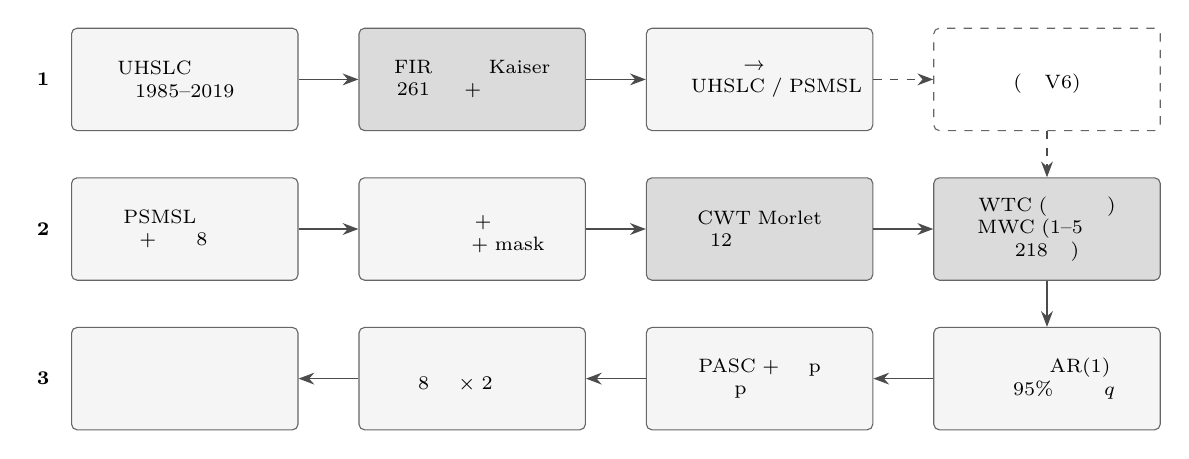
\begin{tikzpicture}[
  box/.style={draw=black!60,fill=black!4,rounded corners=2pt,align=center,font=\scriptsize,
              minimum height=13mm,text width=27mm,inner sep=2.5pt},
  hot/.style={box,fill=black!14},
  arr/.style={-{Stealth[length=2mm]},semithick,black!70},
  lab/.style={font=\scriptsize\bfseries,anchor=east}]
  \def\dx{36.5mm}\def\dy{19mm}
  \node[box] (uh)  at (0,0)          {UHSLC รายชั่วโมง\\1985–2019};
  \node[hot] (fir) at (\dx,0)        {FIR หน้าต่าง Kaiser\\261 แท็ป + ลดอัตราสุ่ม};
  \node[box] (mo)  at (2*\dx,0)      {รายวัน → รายเดือน\\เทียบ UHSLC / PSMSL};
  \node[box,fill=white,dashed] (alt) at (3*\dx,0) {อนุกรมทางเลือก\\(แบบ V6)};
  \node[box] (ps)  at (0,-\dy)       {PSMSL รายเดือน\\+ ดัชนี 8 ตัว};
  \node[box] (pre) at (\dx,-\dy)     {ควบคุมคุณภาพ\\ตัดแนวโน้ม + ฤดูกาล\\เติมช่องว่าง + mask};
  \node[hot] (cwt) at (2*\dx,-\dy)   {CWT Morlet\\12 สเกลต่อออกเทฟ};
  \node[hot] (wtc) at (3*\dx,-\dy)   {WTC (ดัชนีเดี่ยว)\\MWC (1–5 ดัชนี\\218 ชุด)};
  \node[box] (mc)   at (3*\dx,-2*\dy) {มอนติคาร์โล AR(1)\\เกณฑ์ 95\% ปรับตาม $q$};
  \node[box] (pasc) at (2*\dx,-2*\dy) {PASC + ค่า p\\ค่า p ทั้งตระกูล};
  \node[box] (sens) at (\dx,-2*\dy)   {วิเคราะห์ความไว\\8 แบบ × 2 สถานี};
  \node[box] (mech) at (0,-2*\dy)     {เทียบกลไกทางกายภาพ\\จากงานวิจัย};
  \draw[arr] (uh) -- (fir); \draw[arr] (fir) -- (mo); \draw[arr,dashed] (mo) -- (alt);
  \draw[arr,dashed] (alt) -- (wtc);
  \draw[arr] (ps) -- (pre); \draw[arr] (pre) -- (cwt); \draw[arr] (cwt) -- (wtc);
  \draw[arr] (wtc) -- (mc); \draw[arr] (mc) -- (pasc); \draw[arr] (pasc) -- (sens); \draw[arr] (sens) -- (mech);
  \node[lab] at ($(uh.west)+(-1.5mm,0)$) {1};
  \node[lab] at ($(ps.west)+(-1.5mm,0)$) {2};
  \node[lab] at ($(mech.west)+(-1.5mm,0)$) {3};
\end{tikzpicture}
\caption[ขั้นตอนการศึกษา]{ขั้นตอนการศึกษา (1) กรองและลดอัตราสุ่มข้อมูลรายชั่วโมงเพื่อตรวจสอบกับ PSMSL และใช้เป็นอนุกรมทางเลือก
(2) เตรียมสัญญาณรายเดือน คำนวณ CWT, WTC และ MWC ทดสอบนัยสำคัญ และวิเคราะห์ความไว
(3) เปรียบเทียบผลกับกลไกทางกายภาพจากงานวิจัยที่เกี่ยวข้อง}
\label{fig:pipeline}
\end{figure}

% ======================================================================
\section{ผลการศึกษา}

\subsection{ความถูกต้องของการกรองและลดอัตราสุ่ม (Q7)}

ตัวกรอง FIR ที่ออกแบบไว้สามารถกำจัดองค์ประกอบน้ำขึ้นน้ำลงได้ 77–99 dB ซึ่งป้องกันการบิดเบือนขององค์ประกอบฤดูกาลได้ดี
(รูปที่~\ref{fig:filter}) อนุกรมรายเดือนที่ลดอัตราสุ่มแล้ว มีความคลาดเคลื่อนจากข้อมูล PSMSL ในระดับต่ำเพียง 1.1–1.2 มม.
(มัธยฐานของผลต่างสัมบูรณ์ ในช่วงที่ระดับอ้างอิงของข้อมูลคงที่)

\begin{figure}[!htbp]
\centering
\includegraphics[width=0.9\textwidth]{fig02_filter.png}
\caption{ผลตอบสนองเชิงความถี่ของตัวกรอง FIR หน้าต่าง Kaiser (261 แท็ป) เทียบกับความถี่ขององค์ประกอบน้ำขึ้นน้ำลงหลัก}
\label{fig:filter}
\end{figure}

\subsection{ความสัมพันธ์กับดัชนีเดี่ยว: ทะเลอันดามัน (Q1)}

ระดับน้ำทะเลเกาะตะเภาน้อยมีความสัมพันธ์อย่างมีนัยสำคัญกับดัชนี SOI, DMI, WNPMI และ Niño3.4
ในทุกแบบการทดสอบความไวเมื่อพิจารณาทั้งระนาบ ส่วนในช่วงคาบ 2–7 ปี ดัชนี WNPMI อธิบายผลได้สูงสุด (PASC 32.2\%)
(รูปที่~\ref{fig:scorecard} และ~\ref{fig:wtc})

\begin{figure}[!htbp]
\centering
\includegraphics[width=0.9\textwidth]{fig10_scorecard.png}
\caption{PASC ของดัชนีเดี่ยวสำหรับสองสถานีและสองช่วงคาบ ช่องที่มีสีและเครื่องหมาย \tick{} คือมีนัยสำคัญ (p < 0.05) ตัวเลขใต้ค่าแสดงจำนวนแบบการทดสอบความไวที่ยังคงมีนัยสำคัญ}
\label{fig:scorecard}
\end{figure}
\begin{figure}[!htbp]
\centering
\includegraphics[width=\textwidth]{fig03_wtc_maps.png}
\caption{Wavelet coherence ระหว่างระดับน้ำทะเลเกาะตะเภาน้อย (แถวบน) และเกาะหลัก (แถวล่าง) กับดัชนีสามตัว เส้นสีขาวล้อมบริเวณที่เกินเกณฑ์นัยสำคัญ 95\% เส้นประแสดงกรวยอิทธิพล}
\label{fig:wtc}
\end{figure}

\subsection{ความสัมพันธ์กับดัชนีเดี่ยว: อ่าวไทย (Q2)}

ระดับน้ำทะเลเกาะหลักไม่พบ PASC ที่มีนัยสำคัญเหนือระดับสัญญาณรบกวนกับดัชนีใดๆ ทั้งสิ้นในทุกรูปแบบการวิเคราะห์
(รูปที่~\ref{fig:scorecard} และ~\ref{fig:wtc}) ผลลัพธ์ของ PASC แสดงให้เห็นว่า สถานีป้อมพระจุลจอมเกล้า (หลังตัดแนวโน้มการทรุดตัว 15.6 มม./ปี ออก) ไม่มีดัชนีใดให้ผล PASC อย่างมีนัยสำคัญเลย เช่นเดียวกับสถานีเกาะหลัก

\subsection{ลักษณะเชิงเวลาของความสัมพันธ์}

ระดับน้ำฝั่งอันดามันลดต่ำลงอย่างชัดเจนในช่วงที่เกิดเหตุการณ์ El Niño และ IOD บวก
(เช่น ปี 1997–1998 ค่าเฉลี่ยเคลื่อนที่ 12 เดือนลดกว่าปกติราว 210 มม.) แต่สัมประสิทธิ์สหสัมพันธ์แบบทั่วไปตลอดอนุกรมมีค่าต่ำ
ซึ่งสนับสนุนว่าการวิเคราะห์ด้วยเวฟเล็ตให้ภาพที่ชัดเจนกว่า (รูปที่~\ref{fig:events})

\begin{figure}[!htbp]
\centering
\includegraphics[width=\textwidth]{fig11_events.png}
\caption{ระดับน้ำทะเลระหว่างปี (ค่าเฉลี่ยเคลื่อนที่ 12 เดือน) เทียบกับดัชนี Niño3.4 และ DMI ที่กลับเครื่องหมาย ค่า $r$ ใช้เพื่อการบรรยายเท่านั้น}
\label{fig:events}
\end{figure}

\subsection{ความสัมพันธ์เชิงเฟส}

ทิศทางของมุมเฟสสอดคล้องกับกลไกทางกายภาพ ระดับน้ำแปรผันตามทิศทางของดัชนี SOI แต่อยู่ในทิศทางสวนทางกับดัชนี Niño3.4 และ DMI
ขณะที่ดัชนี WNPMI แปรผันในทิศทางเดียวกันโดยระดับน้ำนำหน้าประมาณ 6 เดือน (รูปที่~\ref{fig:phase})

\begin{figure}[!htbp]
\centering
\includegraphics[width=\textwidth]{fig12_phase.png}
\caption{มุมเฟสของ coherence ระหว่างระดับน้ำทะเลเกาะตะเภาน้อยกับดัชนีสี่ตัว (แถบคาบ 2–7 ปี เฉพาะบริเวณที่มีนัยสำคัญ) พื้นที่แรเงาแสดงช่วงทิศที่คาดการณ์จากกลไก}
\label{fig:phase}
\end{figure}

\subsection{เกณฑ์นัยสำคัญของ MWC ตามจำนวนดัชนี (Q6)}

หากไม่มีการปรับเกณฑ์ ค่า PASC จากสัญญาณสุ่มจะพุ่งสูงถึง 97.2\% เมื่อเพิ่มจำนวนดัชนีเป็น 5 ตัว
(รูปแบบเดียวกับที่พบในงานต้นทาง; Song \& Chen, 2022) การปรับเกณฑ์นัยสำคัญให้สัมพันธ์กับจำนวนตัวแปร%
จะช่วยคุมระดับ PASC จากสัญญาณรบกวนไว้ที่ประมาณ 4.7\% ได้อย่างคงที่ (รูปที่~\ref{fig:thr} และ~\ref{fig:false})

\begin{figure}[!htbp]
\centering
\includegraphics[width=0.75\textwidth]{fig05_threshold_vs_q.png}
\caption{เกณฑ์นัยสำคัญที่ระดับ 95\% ของ MWC ตามคาบ สำหรับจำนวนดัชนี 1–5 ตัว}
\label{fig:thr}
\end{figure}
\begin{figure}[!htbp]
\centering
\includegraphics[width=\textwidth]{fig06_q6_false_floor.png}
\caption{PASC เฉลี่ยของดัชนีจริงเทียบกับดัชนีปลอม กรณีไม่ปรับเกณฑ์ (สีแดง) และปรับเกณฑ์ตามจำนวนดัชนี (สีน้ำเงิน) สามเหลี่ยมคือค่าที่ Song และ Chen (2022) รายงาน}
\label{fig:false}
\end{figure}

\subsection{จำนวนและชุดดัชนีที่เหมาะสม (Q3–Q5)}

การใช้ดัชนีเดี่ยวเพียงพอต่อการอธิบายผลลัพธ์แล้ว การเพิ่มจำนวนดัชนีใน MWC แทบไม่ได้เพิ่มอำนาจการอธิบายอย่างมีนัยสำคัญ
(ชุดที่เหมาะสมคือ SOI สำหรับทั้งระนาบ และ WNPMI สำหรับแถบคาบ 2–7 ปี) และแม้ว่าชุดดัชนีประจำภูมิภาคจะมีแนวโน้มอธิบายผลได้ดีกว่า%
ในแถบคาบ 2–7 ปี แต่ยังไม่แข็งแรงพอที่จะเป็นข้อสรุปตายตัว (รูปที่~\ref{fig:best})

\begin{figure}[!htbp]
\centering
\includegraphics[width=\textwidth]{fig07_q3_best_per_q.png}
\caption{PASC ของชุดดัชนีที่ดีที่สุดสำหรับแต่ละจำนวนดัชนี เทียบกับการแจกแจงของค่าสูงสุดจากการค้นหาทั้งตระกูลภายใต้สมมติฐานว่าง}
\label{fig:best}
\end{figure}

\subsection{ความไวต่อการเตรียมข้อมูลและแหล่งข้อมูล}

ข้อสรุปหลักๆ มีความแข็งแรงทนทาน (robust) ในแทบทุกการทดสอบ (รูปที่~\ref{fig:robust}) อย่างไรก็ตาม
ลำดับความสำคัญของดัชนีในช่วงคาบ 2–7 ปีแปรปรวน เนื่องจากข้อมูลของสถานีเกาะตะเภาน้อยระหว่างคลัง PSMSL และ UHSLC
ให้ข้อมูลที่ไม่ตรงกันหลังปี 2005 (ต่างกันประมาณ 10 ซม. ในช่วง 2015–2019) เพราะมีการเปลี่ยนเครื่องมือวัด
การแก้ระดับอ้างอิงที่ไม่ตรงกันระหว่างสองคลัง และพายุทำลายสถานี (University of Hawaii Sea Level Center, 2020)
(รูปที่~\ref{fig:datum})

\begin{figure}[!htbp]
\centering
\includegraphics[width=\textwidth]{fig13_robustness.png}
\caption{ผลของข้อสรุปหลักภายใต้การเตรียมข้อมูลแปดแบบ (V0–V7) ตัวเลขด้านขวาแสดงจำนวนแบบที่ข้อสรุปยังคงมีนัยสำคัญ}
\label{fig:robust}
\end{figure}
\begin{figure}[!htbp]
\centering
\includegraphics[width=\textwidth]{fig14_ktn_datum.png}
\caption{ผลต่างรายเดือนระหว่างข้อมูล PSMSL และ UHSLC ของสถานีเกาะตะเภาน้อย เส้นประแสดงเหตุการณ์ที่มีเอกสารยืนยัน (University of Hawaii Sea Level Center, 2020; Naeije et al., 2022)}
\label{fig:datum}
\end{figure}

% ======================================================================
\section{อภิปรายผล}

\subsection{กลไกทางกายภาพของความสัมพันธ์ฝั่งทะเลอันดามัน}

ปรากฏการณ์ El Niño และ IOD ฝั่งบวกกระตุ้นลมเหนือเส้นศูนย์สูตร ซึ่งก่อให้เกิดคลื่นเคลวิน (Ashok et al., 2003)
คลื่นนี้เคลื่อนตัวมายังชายฝั่งทะเลอันดามัน ส่งผลให้ระดับน้ำลดต่ำลงในทิศทางและจังหวะเวลาที่สอดคล้องกัน
(Han \& Webster, 2002; Rao et al., 2010) ดัชนีทั้งสี่ตัวส่งผลกระทบผ่านตัวแปรตัวกลางนี้ตัวเดียวกัน
จึงทำให้การรวมดัชนีเข้าด้วยกันไม่ได้ช่วยเพิ่มข้อมูลใหม่ (รูปที่~\ref{fig:mech})

\begin{figure}[!htbp]
\centering
\includegraphics[width=\textwidth]{map03_mechanism.png}
\caption{ลำดับกลไกในปีที่เกิด El Niño หรือ IOD บวก เรียบเรียงจาก Han และ Webster (2002), Rao et al. (2010), Aparna et al. (2012), Brown et al. (2019), Anutaliya (2023) และ นิพนธ์ พงศ์สุวรรณ (2564)}
\label{fig:mech}
\end{figure}

\subsection{การไม่ปรากฏความสัมพันธ์ในอ่าวไทย}

อ่าวไทยมีสภาพทางกายภาพเป็นอ่าวตื้นที่ตอบสนองต่อลมท้องถิ่นและมรสุมได้ทันที (Anutaliya, 2023)
นอกจากนี้ยังตั้งอยู่นอกเส้นทางการเคลื่อนตัวของคลื่นเคลวิน (ท่อนำคลื่น) (Liu et al., 2011)
และสัญญาณ ENSO ที่มีขนาดเล็กมากมักจะถูกกลบด้วยความแปรปรวนของวัฏจักรฤดูกาล (Luu et al., 2015) (รูปที่~\ref{fig:twoseas})

\begin{figure}[!htbp]
\centering
\includegraphics[width=0.72\textwidth]{map02_two_seas.png}
\caption{สรุปผลเชิงพื้นที่ของสองสถานีพร้อมความลึกของพื้นท้องทะเล}
\label{fig:twoseas}
\end{figure}

\subsection{นัยต่อการใช้ MWC และการเปรียบเทียบกับงานต้นทาง}

การเพิ่มดัชนีใน MWC โดยไม่ระวังเกณฑ์นัยสำคัญ อาจทำให้สัญญาณรบกวนถูกตีความว่าเป็นความสัมพันธ์จริง
งานวิจัยต่อยอดจึงควรปรับเกณฑ์ตามจำนวนตัวแปร $q$ อย่างรัดกุมเสมอ

\subsection{ความไม่แน่นอนจากข้อมูลมาตรวัด}

ข้อจำกัดจากความคลาดเคลื่อนของข้อมูลหลังปี 2005 ทำให้ไม่สามารถยืนยันได้ว่า WNPMI คือดัชนีเด่นที่สุด
สรุปได้เพียงว่าระดับน้ำฝั่งอันดามันสัมพันธ์กับโหมด ENSO และมรสุม/มหาสมุทรอินเดีย

% ======================================================================
\section{สรุปและข้อเสนอแนะ}

\subsection{สรุปผลการศึกษา}

\begin{itemize}
  \item ระดับน้ำทะเลฝั่งอันดามันสัมพันธ์อย่างชัดเจนกับ ENSO และ IOD สอดคล้องกับกลไกของคลื่นเคลวิน
  \item อ่าวไทยไม่พบการตอบสนองต่อดัชนีใดๆ เกินระดับสัญญาณรบกวน
  \item ทิศทางการแปรผันสอดคล้องตามทฤษฎีกลไกทางกายภาพ
  \item การใช้ MWC รวมหลายดัชนีไม่ได้มีประโยชน์ไปกว่าการพิจารณาดัชนีเดี่ยว
\end{itemize}

\subsection{ข้อจำกัดของการศึกษา}

\begin{itemize}
  \item การวัดค่า Coherence ไม่สามารถยืนยันความเป็นเหตุเป็นผล (causation) ได้
  \item คลังข้อมูลหลังปี 2005 มีปัญหาความไม่สอดคล้องกันที่หาข้อสรุปชี้ขาดไม่ได้
  \item การวิเคราะห์แถบคาบทศวรรษ (8–16 ปี) ทำได้ยากเนื่องจากหน้าต่างเวลาข้อมูลที่มีจำกัด
\end{itemize}

\subsection{ข้อเสนอแนะสำหรับการศึกษาต่อ}

\begin{itemize}
  \item นำข้อมูลความสูงผิวน้ำทะเลจากดาวเทียมมาเทียบสอบแก้ปัญหาความคลาดเคลื่อนของมาตรวัด
  \item ประยุกต์ใช้ partial wavelet coherence ควบคุมอิทธิพลร่วมของดัชนี
  \item วิเคราะห์อ่าวไทยแยกช่วงฤดูเพื่อให้เห็นสัญญาณ ENSO ที่ชัดเจนขึ้น
\end{itemize}

% ======================================================================
\centerheading{เอกสารอ้างอิง}

\begingroup
\setlength{\parindent}{0pt}
\setlength{\parskip}{0.3em}
\everypar{\hangindent=2em\hangafter=1}   % ย่อหน้าแบบแขวน (hanging indent) ตาม APA
\small

นิพนธ์ พงศ์สุวรรณ. (2564). \textit{ผลกระทบจากปรากฏการณ์น้ำลงมากผิดปกติต่อแนวปะการังทางฝั่งทะเลอันดามัน}.
กรมทรัพยากรทางทะเลและชายฝั่ง.

Anutaliya, A. (2023). Surface circulation in the Gulf of Thailand from remotely sensed observations: Seasonal and interannual
timescales. \textit{Ocean Science, 19}, 335–350.

Aparna, S. G., McCreary, J. P., Shankar, D., \& Vinayachandran, P. N. (2012). Signatures of Indian Ocean Dipole and
El Niño–Southern Oscillation events in sea level variations in the Bay of Bengal. \textit{Journal of Geophysical Research, 117}, C10012.

Ashok, K., Guan, Z., \& Yamagata, T. (2003). A look at the relationship between the ENSO and the Indian Ocean Dipole.
\textit{Journal of the Meteorological Society of Japan, 81}(1), 41–56.

Brown, B. E., Dunne, R. P., Somerfield, P. J., Edwards, A. J., Simons, W. J. F., Phongsuwan, N., Putchim, L., Anderson, L.,
\& Naeije, M. C. (2019). Long-term impacts of rising sea temperature and sea level on shallow water coral communities over
a \textasciitilde 40 year period. \textit{Scientific Reports, 9}, 8826.

Grinsted, A., Moore, J. C., \& Jevrejeva, S. (2004). Application of the cross wavelet transform and wavelet coherence to
geophysical time series. \textit{Nonlinear Processes in Geophysics, 11}, 561–566.

Han, W., \& Webster, P. J. (2002). Forcing mechanisms of sea level interannual variability in the Bay of Bengal.
\textit{Journal of Physical Oceanography, 32}, 216–239.

Hu, W., \& Si, B. C. (2016). Technical note: Multiple wavelet coherence for untangling scale-specific and localized
multivariate relationships in geosciences. \textit{Hydrology and Earth System Sciences, 20}, 3183–3191.

Liu, Q., Feng, M., \& Wang, D. (2011). ENSO-induced interannual variability in the southeastern South China Sea.
\textit{Journal of Oceanography, 67}, 127–133.

Luu, Q. H., Tkalich, P., \& Tay, T. W. (2015). Sea level trend and variability around Peninsular Malaysia.
\textit{Ocean Science, 11}, 617–628.

Maraun, D., \& Kurths, J. (2004). Cross wavelet analysis: Significance testing and pitfalls.
\textit{Nonlinear Processes in Geophysics, 11}, 505–514.

Naeije, M. C., et al. (2022). Monitoring megathrust-earthquake-cycle-induced relative sea-level changes near Phuket,
South Thailand, using (space) geodetic techniques. \textit{Remote Sensing, 14}, 5145.

Permanent Service for Mean Sea Level. (n.d.). \textit{Station 446 Ko Taphao Noi; Station 174 Ko Lak; Station 444 Fort
Phrachula Chomklao}. https://psmsl.org

Rao, R. R., Girish Kumar, M. S., Ravichandran, M., Rao, A. R., Gopalakrishna, V. V., \& Thadathil, P. (2010). Interannual
variability of Kelvin wave propagation in the wave guides of the equatorial Indian Ocean, the coastal Bay of Bengal and the
southeastern Arabian Sea during 1993–2006. \textit{Deep-Sea Research Part I, 57}(1), 1–13.

Song, C., \& Chen, X. (2022). Multivariate analysis of multiscale periodicity in North American annual mean sea level based on
wavelet coherence and multiple wavelet coherence. \textit{Journal of Water and Climate Change, 13}(9), 3435–3457.

Torrence, C., \& Compo, G. P. (1998). A practical guide to wavelet analysis.
\textit{Bulletin of the American Meteorological Society, 79}(1), 61–78.

Torrence, C., \& Webster, P. J. (1999). Interdecadal changes in the ENSO–monsoon system. \textit{Journal of Climate, 12}, 2679–2690.

University of Hawaii Sea Level Center. (2020). \textit{Research quality data documentation: Station 148A Ko Taphao Noi} (qa148a.dmt).

Wouters, B., \& Chambers, D. P. (2010). Analysis of seasonal ocean bottom pressure variability in the Gulf of Thailand from
GRACE. \textit{Global and Planetary Change, 74}(2), 76–81.

\endgroup

\end{document}
